\section{Real-only SHAP descriptor analysis}\label{sec:shap}

SHAP values~\cite{shap2017} are computed with \texttt{TreeExplainer}~\cite{treeshap2020}
on the final real-only interpretation model fitted to all 118 usable observations (Sec.~\ref{sec:methods}). One-hot columns are
reported individually and aggregated back to the parent descriptor by summing $|$SHAP$|$
within each row before averaging. This is an \emph{association} analysis within the compiled
corpus, not a causal or predictive claim.

\subsection{Descriptor ranking}
Table~\ref{tab:shap} and Fig.~\ref{fig:shapimp} give the ranking. The five leading
descriptors, with their share of total attribution, are: composition family (22\%); H\textsubscript{2}SO\textsubscript{4} concentration (M) (20\%); scan rate (mV\,s\textsuperscript{-1}) (16\%); interlayer spacing (\AA) (10\%); layer morphology (9\%). The ranking agrees closely with
the independent fold-wise held-out SHAP computed during cross-validation: the top five
descriptors each entered the fold-level top five in
80--100\%
of folds.

\subsection{Direction of the associations}
Fig.~\ref{fig:shapbee} and Fig.~\ref{fig:shapdep} show directionality. Higher
H\textsubscript{2}SO\textsubscript{4} concentration is associated with higher predicted
capacitance ($\rho = +0.72$ between the
descriptor value and its own SHAP value), consistent with greater proton availability for
Ti--O pseudocapacitance~\cite{lukatskaya2017}. Higher scan rate is associated with lower predicted capacitance
($\rho = -0.93$), consistent with
rate-limited ion access to the interlayer galleries.

\paragraph{A trend that contradicts the naive expectation.} Interlayer spacing is associated
with \emph{lower} predicted capacitance
($\rho = -0.75$), the opposite of the expectation that a wider gallery eases ion
access. We do not report this as a physical finding. Two confounds are more plausible: the
largest reported $d$-spacings in this corpus belong predominantly to pillared and composite
architectures whose \emph{gravimetric} capacitance is diluted by the mass of the
intercalant, and $d$-spacing is conventionally measured on a dry film rather than in the
hydrated, polarised state in which charge is actually stored. This is a concrete illustration
of why a monotonicity prior must not be read off a SHAP plot.

\paragraph{The confounding caveat, stated quantitatively.} Sec.~\ref{sec:domainshift}
showed that several descriptors are paper-level constants. Electrolyte molarity, the
second-ranked descriptor, has ICC$(1) = 1.00$: it does not vary at
all within a publication. Its SHAP attribution therefore cannot be statistically separated
from the identity of the publications that used each molarity, and the same applies to
interlayer spacing (\AA), current density (A\,g\textsuperscript{-1}), electrode thickness ($\upmu$m) and specific surface area (m\textsuperscript{2}\,g\textsuperscript{-1}). The ranking
should be read as ``descriptors along which the corpus is organised and which the model
exploits'', not as ``levers that would change capacitance if turned''. Distinguishing the two
requires controlled experiments that vary one descriptor within a single laboratory
protocol --- which is precisely what the corpus lacks.

\begin{figure}[htbp]\centering
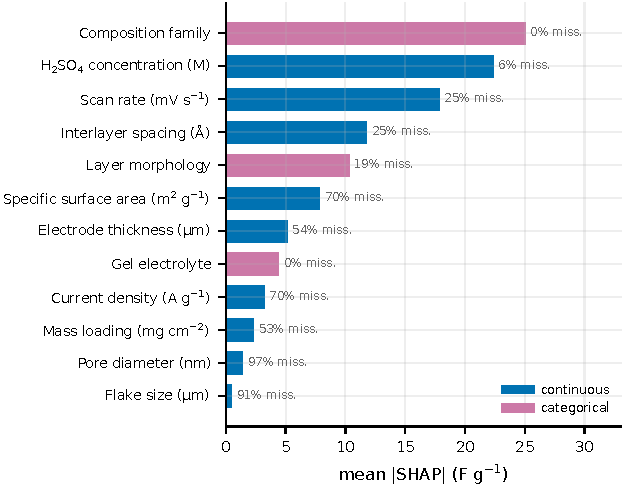
\includegraphics[width=\columnwidth]{figures/fig06_real_shap_importance.pdf}
\caption{Descriptor-level SHAP importance of the final real-only interpretation model.
Bars are the mean absolute SHAP value; annotations give the fraction of observations for
which the descriptor is not reported.}
\label{fig:shapimp}\end{figure}

\begin{figure}[htbp]\centering
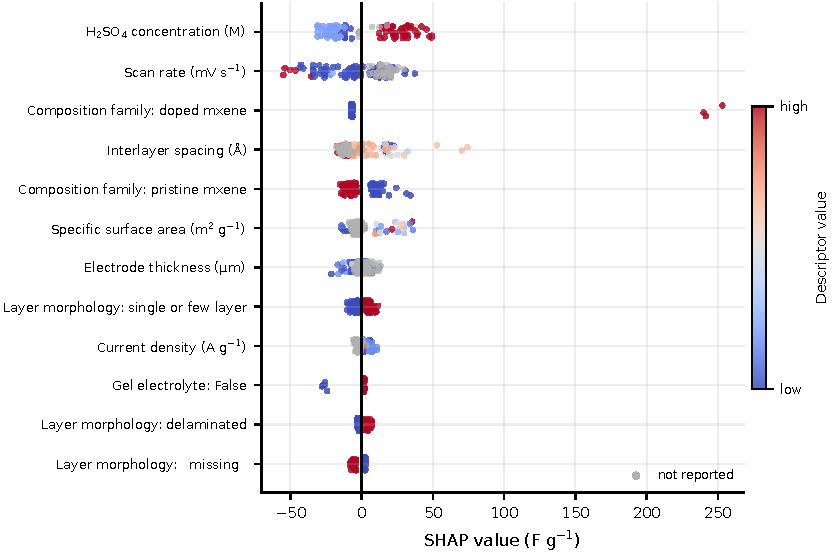
\includegraphics[width=\columnwidth]{figures/fig07_real_shap_beeswarm.pdf}
\caption{SHAP value distribution per encoded feature, coloured by descriptor value. Grey
points are observations for which the descriptor is not reported.}
\label{fig:shapbee}\end{figure}

\begin{figure*}[htbp]\centering
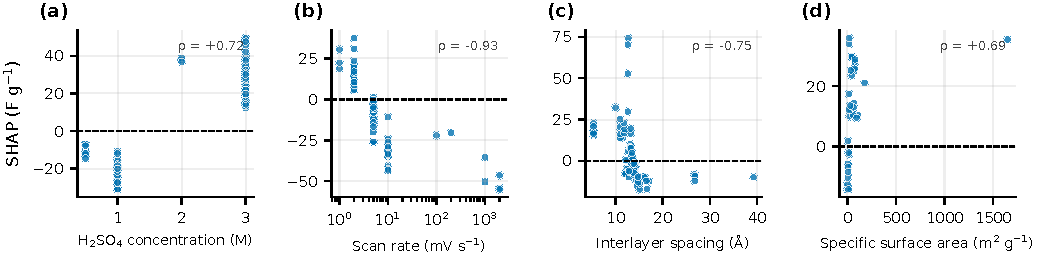
\includegraphics[width=\textwidth]{figures/fig07b_real_shap_dependence.pdf}
\caption{SHAP dependence for the leading continuous descriptors. $\rho$ is the Spearman
correlation between the descriptor value and its own SHAP contribution. The negative trend in
interlayer spacing runs against the naive physical expectation and is discussed in the text.}
\label{fig:shapdep}\end{figure*}

\begin{table}[htbp]
\centering
\caption{Descriptor-level SHAP attribution of the final real-only interpretation model fitted to all usable real observations. $\overline{|\mathrm{SHAP}|}$ in F\,g\textsuperscript{-1}; share, missingness and top-5 frequency in per cent.}
\label{tab:shap}
\footnotesize
\begin{tabular}{rlrrrrrrr}
\toprule
\textbf{Rank} & \textbf{Descriptor} & \textbf{$\overline{|\mathrm{SHAP}|}$} & \textbf{Share} & \textbf{Miss.} & \textbf{Fold rank} & \textbf{Rank SD} & \textbf{Top-5} & \textbf{$\rho$} \\
\midrule
1 & Composition family & 25.05 & 22.3 & 0 & 2.4 & 0.89 & 100 & -- \\
2 & H\textsubscript{2}SO\textsubscript{4} conc.\ (M) & 22.37 & 19.9 & 6 & 1.4 & 0.89 & 100 & 0.72 \\
3 & Scan rate (mV\,s$^{-1}$) & 17.87 & 15.9 & 25 & 2.8 & 1.10 & 100 & -0.93 \\
4 & Interlayer spacing (\AA) & 11.78 & 10.5 & 25 & 4.0 & 1.58 & 80 & -0.75 \\
5 & Layer morphology & 10.31 & 9.2 & 19 & 4.8 & 0.45 & 100 & -- \\
6 & Specific surface area (m$^2$\,g$^{-1}$) & 7.85 & 7.0 & 70 & 6.4 & 1.52 & 20 & 0.69 \\
7 & Electrode thickness ($\upmu$m) & 5.14 & 4.6 & 54 & 7.0 & 1.00 & 0 & -0.23 \\
8 & Gel electrolyte & 4.43 & 3.9 & 0 & 10.0 & 2.00 & 0 & -- \\
9 & Current density (A\,g$^{-1}$) & 3.23 & 2.9 & 70 & 7.8 & 1.48 & 0 & 0.04 \\
10 & Mass loading (mg\,cm$^{-2}$) & 2.33 & 2.1 & 53 & 9.6 & 0.89 & 0 & -0.07 \\
\bottomrule
\end{tabular}
\par\vspace{2pt}\begin{minipage}{\linewidth}\scriptsize ``Fold rank'' and ``Rank SD'' come from the independent held-out SHAP computation of the paper-grouped cross-validation; ``Top-5'' is the fraction of folds in which the descriptor entered the five most important. $\rho$ is the Spearman correlation between a descriptor's value and its own SHAP value (direction of the association, not a causal claim); it is defined for continuous descriptors only.\end{minipage}
\end{table}
